%% 
%% Copyright 2019 Elsevier Ltd
%% 
%%
%%%%%%%%%%%%%%%%%%%%%%%%%%%% ! ! ! SUBMISSION CHECKLIST ! ! ! %%%%%%%%%%%%%%%%%%%%%%%%%%%%
%%
%% Please confirm that your submission follows all the requirements of the guidelines, including the submission checklist:
%% _ Cover letter
%% _ Highlights
%% _ Authorship statement
%% _ The manuscript must be single column and double spaced
%% _ Reference must be in the author-date format
%% _ Code availability section 
%%
%% *All the manuscripts in disagreement with the guidelines will be desk-rejected without editorial check.
%%
%% --------------------------------------
%%
%% This file is part of the 'CAS Bundle'.
%%  
%% It may be distributed under the conditions of the LaTeX Project Public
%% License, either version 1.2 of this license or (at your option) any
%% later version.  The latest version of this license is in 
%%    http://www.latex-project.org/lppl.txt 
%% and version 1.2 or later is part of all distributions of LaTeX
%% version 1999/12/01 or later.
%%   
%% The list of all files belonging to the 'CAS Bundle' is
%% given in the file `manifest.txt'.
%% 
%% Template article for cas-dc documentclass for  
%% double column output.
 
%\documentclass[a4paper,fleqn,longmktitle]{cas-dc}
\documentclass[a4paper,fleqn]{cas-sc}

\usepackage[authoryear]{natbib}
\usepackage{graphicx} 
\usepackage{float}
\usepackage{algorithm}  
\usepackage{algpseudocode}
\usepackage{color}
\usepackage{setspace}
\usepackage[nomarkers,figuresonly]{endfloat}


\newcommand{\colorComments}{black} 
 
%%%Author definitions
\def\tsc#1{\csdef{#1}{\textsc{\lowercase{#1}}\xspace}}
\tsc{WGM}
\tsc{QE}
\tsc{EP}
\tsc{PMS}
\tsc{BEC}
\tsc{DE}
%%%

\usepackage{lineno}
\linenumbers 

\begin{document}
\let\WriteBookmarks\relax
\def\floatpagepagefraction{1}
\def\textpagefraction{.001}
\shorttitle{Short title}
\shortauthors{Polat A.}

\title [mode = title]{A Fast Method for Detecting Rock Blocks and Calculating Volumes and 3D Surface Areas}


\author[0]{Ali Polat}[orcid=0000-0002-9147-3633]
%\credit{ Author 1 contribution  }

%\author[2]{Author 2} 
%\credit{Author 2 contribution }



\address[0]{Provincial Directorate of Disaster and Emergency, 58000, Sivas, Turkey}
%\address[2]{Author 2 affiliation}


\begin{abstract}
Rockfall events are a type of natural disaster that causes loss of life and property in the world. The risk of rockfall can be eliminated by using rockfall prevention methods. To choose the most suitable method, projecting studies should be carried out. This study aims to automatically detect rock blocks in a region and calculate their volumes and 3D surface areas. For this purpose, U-Net segmentation method and Python software language were used. DenseNet121 transfer learning method based on convolutional neural networks was used for feature extraction. The data set was created from the orthophoto images obtained by an unmanned aerial vehicle (UAV). Using the random sampling method, 369 images were selected for training and 191 images for test. As a result of the analysis, the IOU (Intersection Over Union) was calculated as 85\% for training and 84\% for test. The trained model was applied to the study area and 3111 rock blocks were detected. The resulting map is saved as a vector file with coordinates and can be opened in any GIS software. The volumes and 3D surface areas of the rock blocks were calculated with Python script as 275.93 m$^3$ and 2615.23 m$^2$, respectively. With this study, rock blocks can be detected automatically, and their volumes and 3D surface areas can be measured. These results can be used in the selection of rockfall prevention methods. In addition, the codes used in this study can automatically detect different geological formations from aerial photographs. Also, volume and 3D surface area algorithms developed in this study can be used to calculate different types of objects.
\end{abstract}
 



\begin{keywords}
Convolutional Neural Networks \sep 3D Surface Area Calculation \sep Volume Calculation\sep  Rock segmentation \sep  Rockfall\sep U-Net
\end{keywords}

\maketitle 

\printcredits

\doublespacing


\section{Introduction}
\label{intro}
In many parts of the world, loss of life and property is experienced, and large-scale economic losses occur due to natural disasters. One of these natural disasters is rockfall events. Rockfalls are a type of slope instability in which blocks of rock confined to discontinuities move very rapidly from the source region \citep{varnes1978slope, hutchinson1988morphological, CrudenVarnes1996}. Due to the high velocity during the event, rockfalls can be very dangerous for structures in their route depending on the block size. Although it is a type of disaster that affects small areas, its consequences can be very serious. That's why rockfall prevention studies are important. There are studies on this subject in the literature \citep{liu2021trajectory, keskin2022kinematic,ji2023assessment,kainthola2023stability, cao2024risk}. Some preliminary studies are needed to develop a prevention method. One of them is the detection of rock blocks and the calculation of their geometric properties. In this study, rock blocks were segmented, and their volumes and 3D surface areas were calculated. 

There are various studies on rock segmentation in the literature. \cite{dunlop2006automatic} developed a technique for the characterization of rocks using albedo, color, texture, and shape features. In that work, rocks in natural scenes were segmented and located with accurate boundaries. For segmentation purpose top-down and bottom-up knowledge are combined, and geologic rock analysis performed successfully.

In the study conducted by \cite{Song2006AFF}, rock segmentation on Mars was performed to plan routes and determine landing areas. Texture-based image segmentation and edge-flow driven active contour has been developed. Wavelet based local transform, multi-resolution histograms, and inter-scale decision were combined and used for rock segmentation. As a result of the experiments, \cite{Song2006AFF} obtained reliable rock segmentation results.

The place of visual navigation in planetary rover autonomy is crucial. Rock segmentation is an important and challenging task for rover autonomy due to the high computational load and real-time requirement. \cite{kuang2021rock} propose a rock segmentation network (NI-U-Net++) to aid in the visual navigation of rovers. The created model consists of two steps. In the first step, called pre-training, synthetic rock images are generated and used to pre-train the NI-U-Net++ network. In the second phase, transfer-training, the pre-trained NI-U-Net++ network is fine-tuned using real-life images.

\cite{guo2022method} proposed an adaptive watershed segmentation method based on distance transformation for blasted rock piles images. They obtained 95.65\% segmentation accuracy for limestone and granite rock blocks with area over 100 cm$^2$. 

Segmentation of rocks is important in mining as well as in geology. Segmentation is used in this area to determine the size distribution of rock fragments, to organize and optimize blasting, and to reduce environmental impact. For this purpose, \cite{malladi2014superpixels} proposed a simple superpixel algorithm called Superpixels Using Morphology (SUM), which uses a watershed transformation approach to generate superpixels; and made a study comparing some of the current superpixel algorithms on rock images.

Recently, various deep learning and machine learning algorithms, including Convolutional Neural Networks (CNN), have been proposed by researchers working on rock segmentation. \cite{karimpouli2019segmentation} used convolutional autoencoder networks called SegNet for segmentation of digital rock images. Due to the limited number of rock images, cross-correlation based simulation was applied to increase the number of images. 20 images taken from Berea sandstone were used as dataset. As a result of the experiments, they obtained an accuracy value of 96\%.

\cite{xue2021rock} made rock segmentation study for a different purpose; they proposed the rock segmentation visual system to assist Tunnel Boring Machine (TBM) driving. TBM is an essential equipment for digging long-range tunnels. They applied different deep learning network for semantic segmentation of rocks.

In the above studies, rock segmentation was carried out for different purposes. In this study, rock segmentation was carried out as a necessary preliminary study in the development of rockfall prevention methods. Rock blocks were detected precisely in a fast, economical, and safe manner. In addition, the volumes and 3D surface areas of rock blocks were calculated. The methods and algorithms used in the study can be used in many fields such as engineering applications, and geological-geomorphological studies.

\subsection{Study area}
The study area is in the north of Karasar village, which is approximately 156 km away from Sivas city (Fig. \ref{fig:Figure1}). This area consists of Middle Miocene aged agglomerate and tuff units (MTA 1/25000) (Fig. \ref{fig:Figure2}). This unite was defined as Adatepe volcanites according to \cite{yilmaz2004divriugi}. The unit consists of black, red-brown, and brown-black colored basaltic lava flows and less commonly agglomerate and tuffs. The rock blocks in this unit expose a risk of rockfall. Lower Miocene aged sandstone-mudstone-limestone units are observed in the settlement area (Karasar village) and vicinity.
\begin{figure}
	\centering
	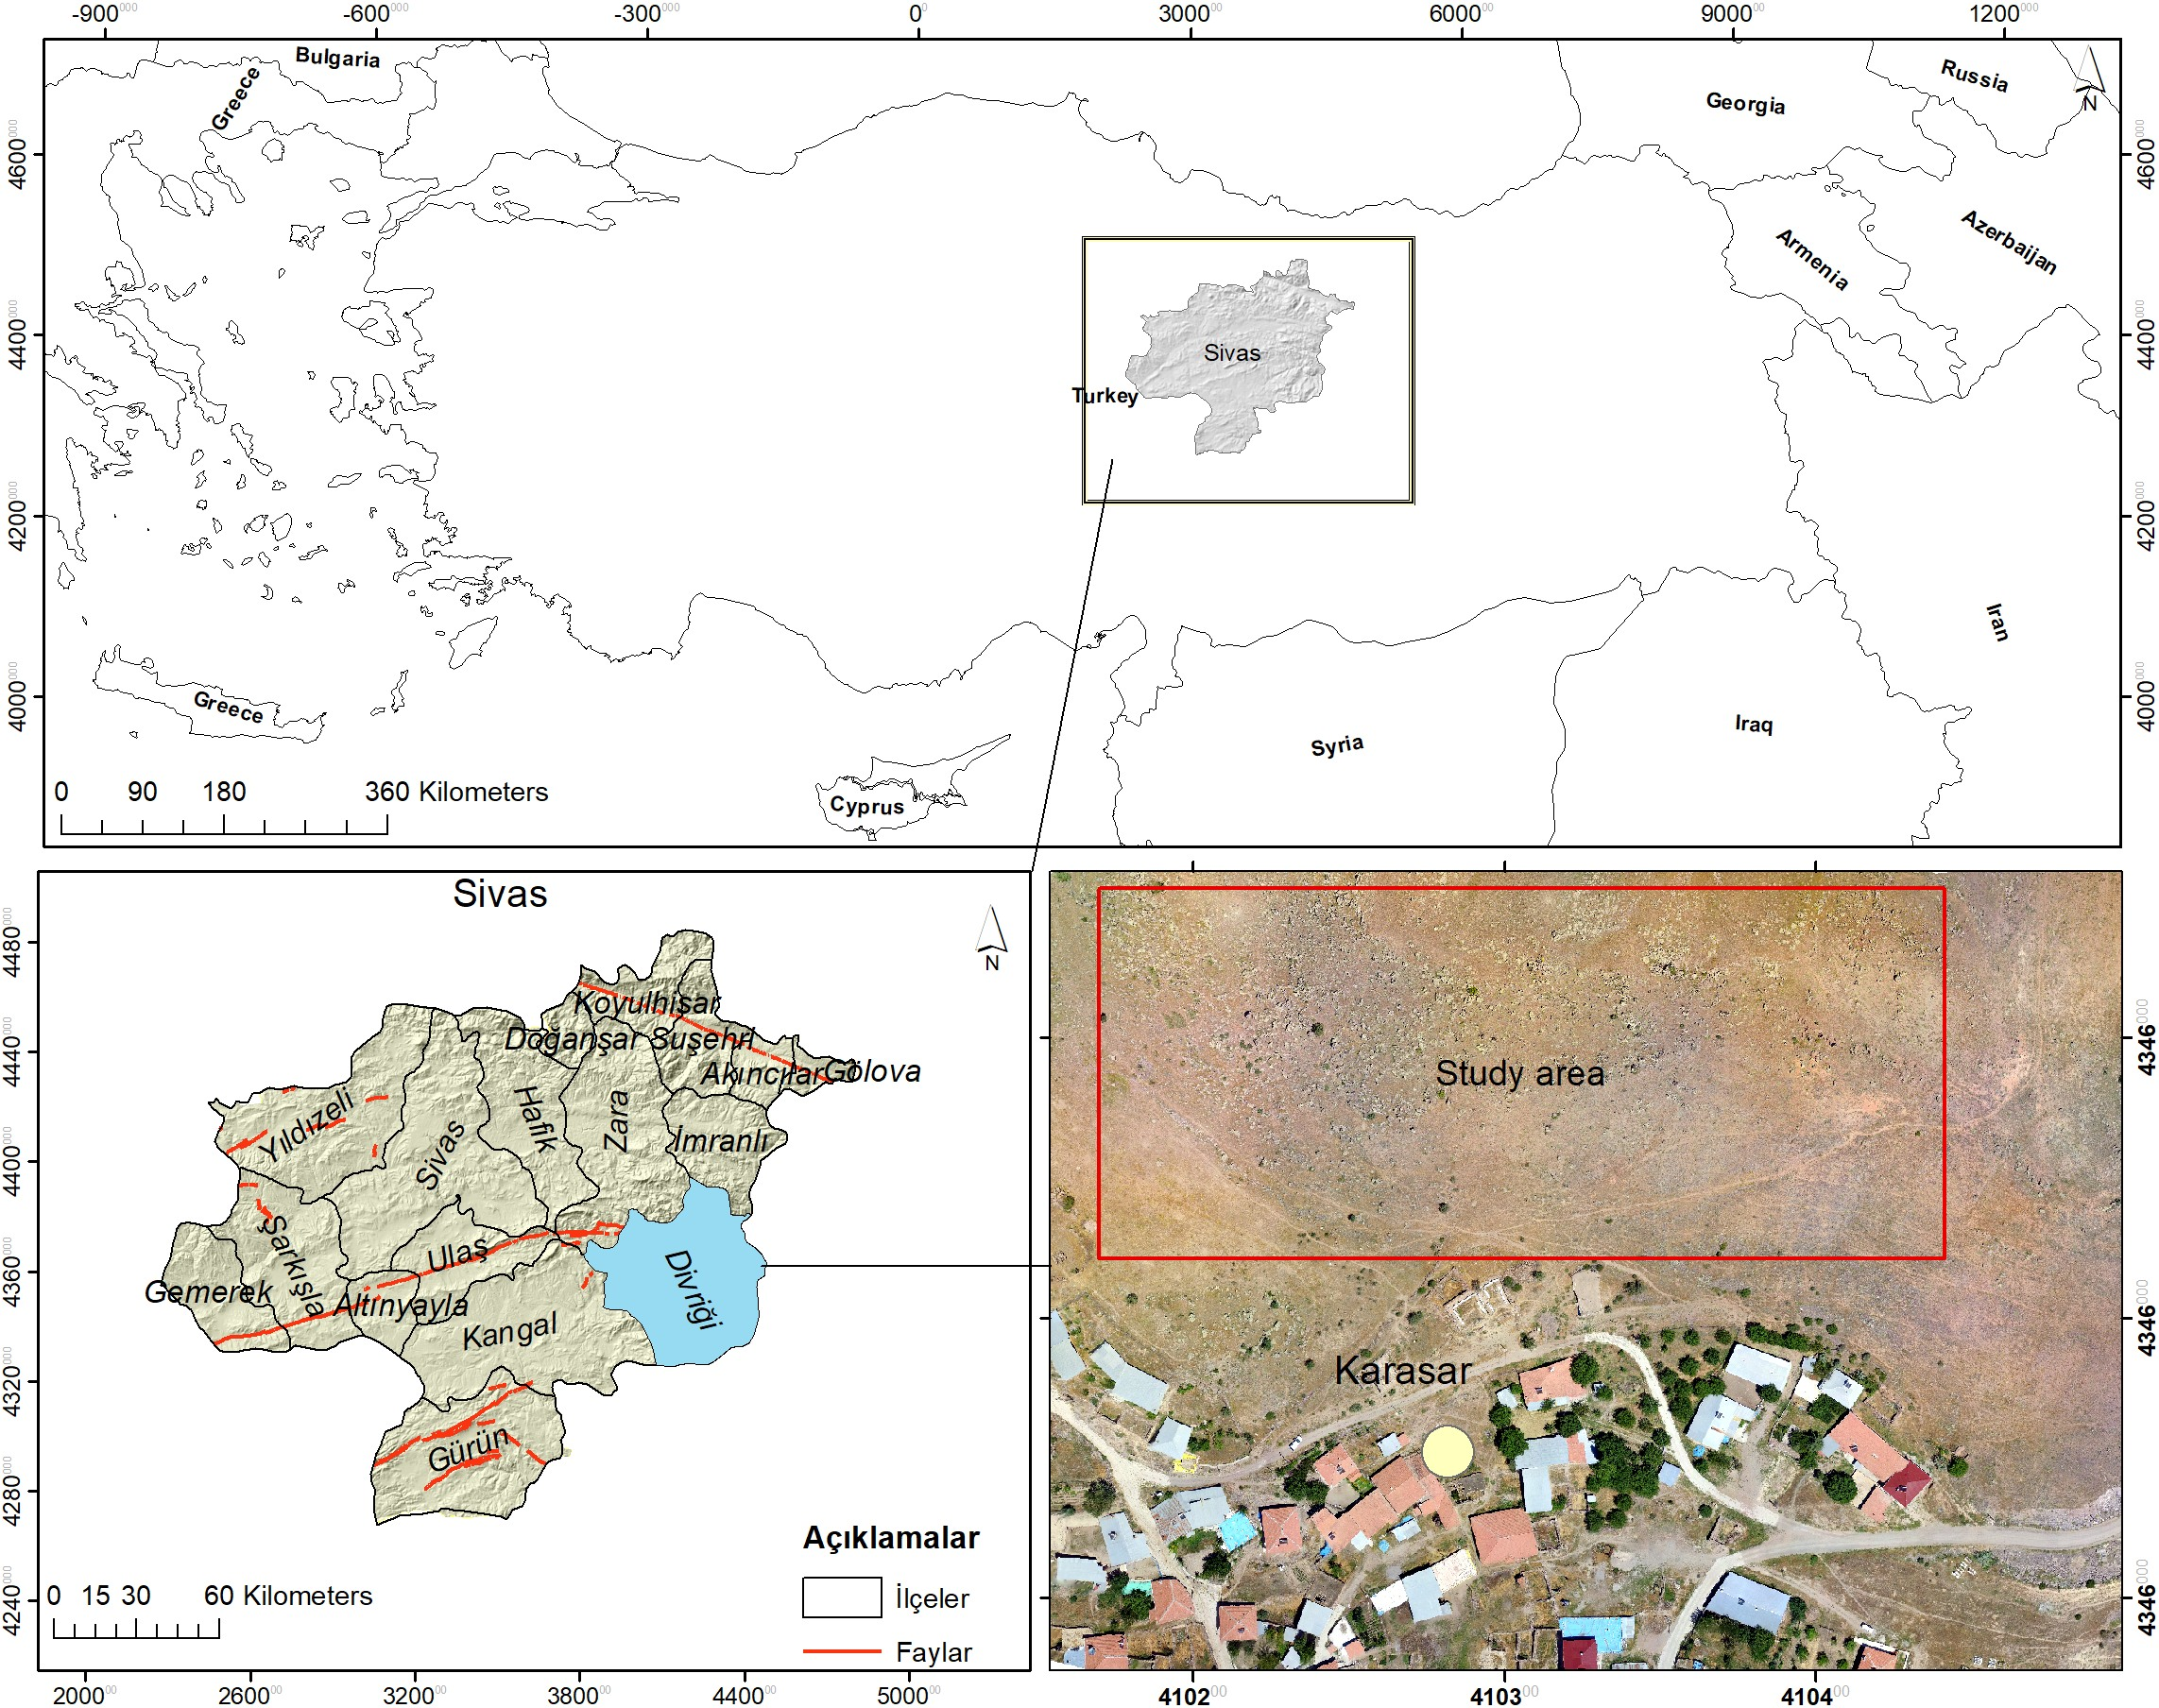
\includegraphics[width=0.75\textwidth]{figures/fig1.jpg}
	\caption{ Location map}
	\label{fig:Figure1}
\end{figure}

Karasar village is located on the slopes of a hill. The bedrock on the hill is heavily fractured and cracked. There are many rock blocks that have fallen from the upper parts of the slope. The sizes of these blocks vary from 0.5 m$^3$ to 15 m$^3$. Rapid temperature changes, heavy snow and precipitation, freeze-thaw cycles, earthquakes, and human-induced factors increase the risk of rockfall in the region.
\begin{figure}[pos=h]
	\centering
	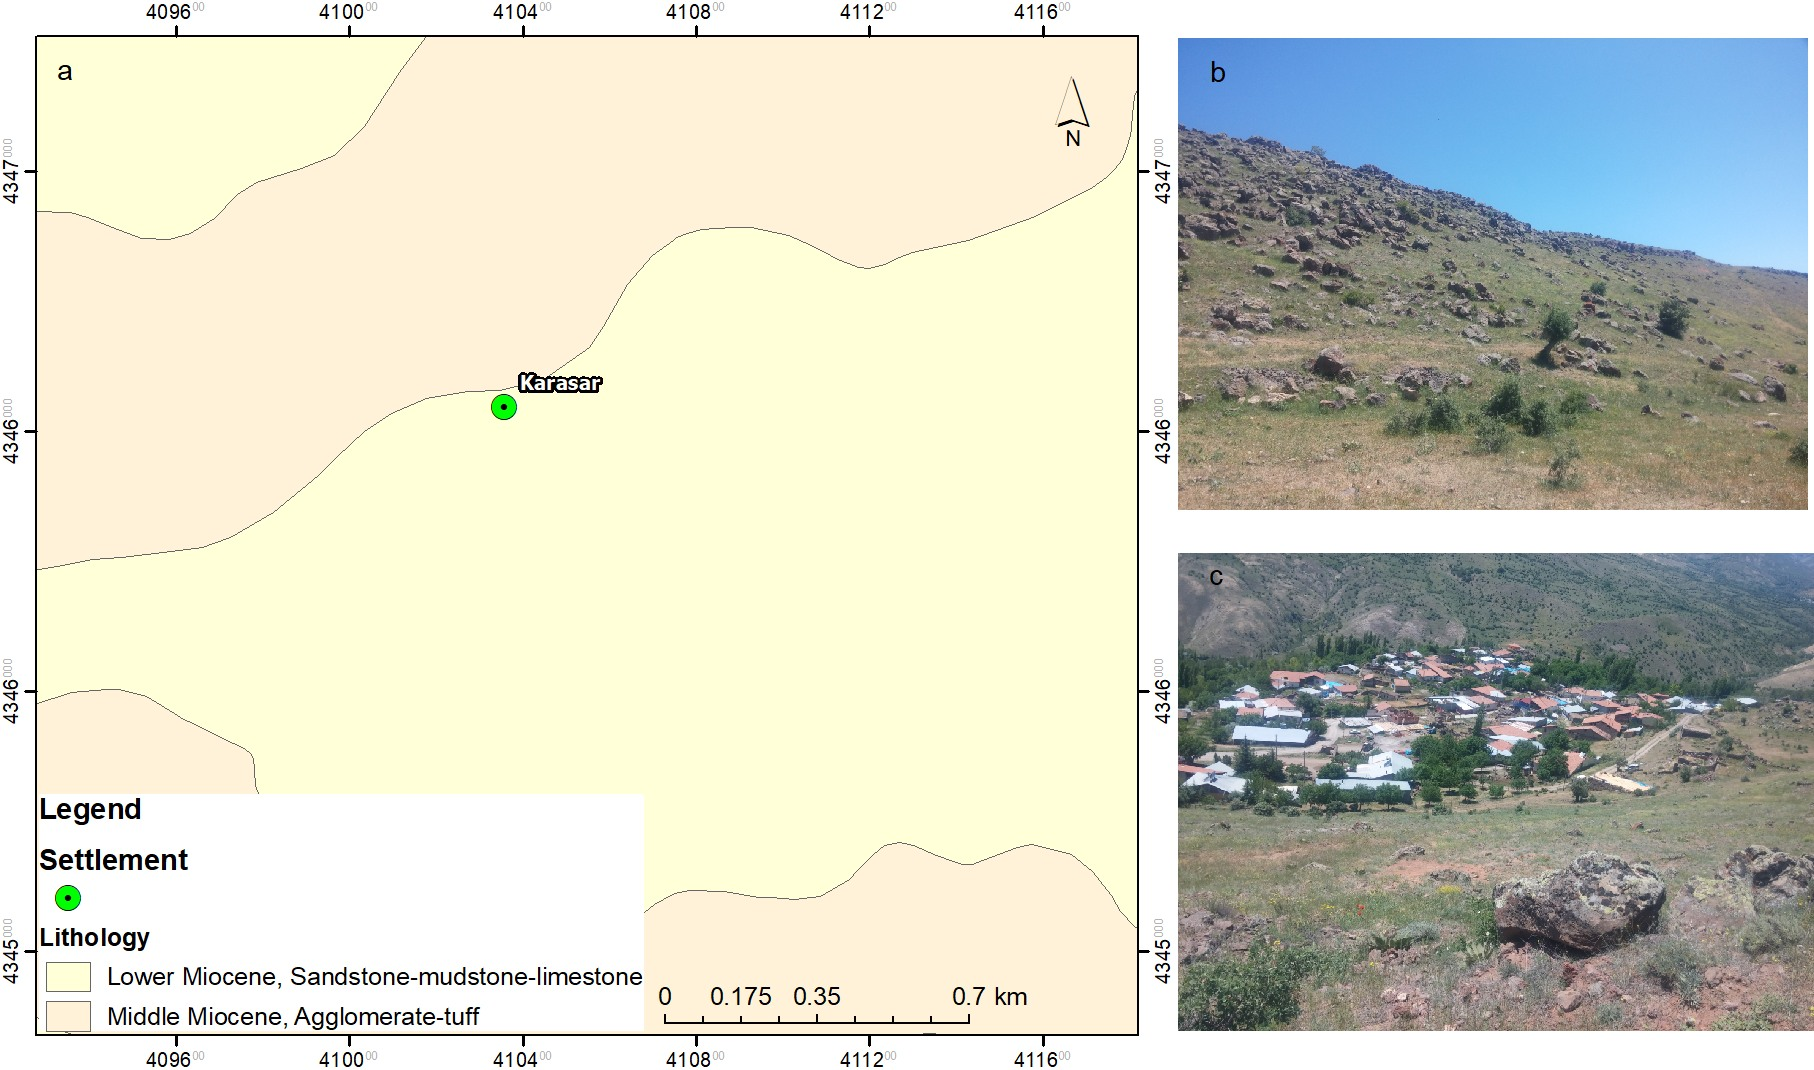
\includegraphics[width=0.75\textwidth]{figures/fig2.jpg}
	\caption{ Geological map (1/25000 scale geological map of General Directorate of Mineral Research and Explorations) (a), rock blocks (b), settlement and rocks (c)}
	\label{fig:Figure2}
\end{figure}

\section{Methodology}
Creating the dataset is a big problem for classification or segmentation processes. In this study, Unmanned Air Vehicle (UAV) was used to collect data. An orthophoto image of the region was created from aerial photographs obtained by UAV.Model building processes were conducted in a part of the study area. Training and testing images were generated from this region. Rock blocks were labeled, and mask images were created. The segmentation process was then carried out using Python and necessary libraries, and the results were converted into polygon vector files. Additionally, the volumes and 3D surface areas of all the rocks were calculated (Fig. \ref{fig:Figure3}).

\begin{figure}
	\centering
	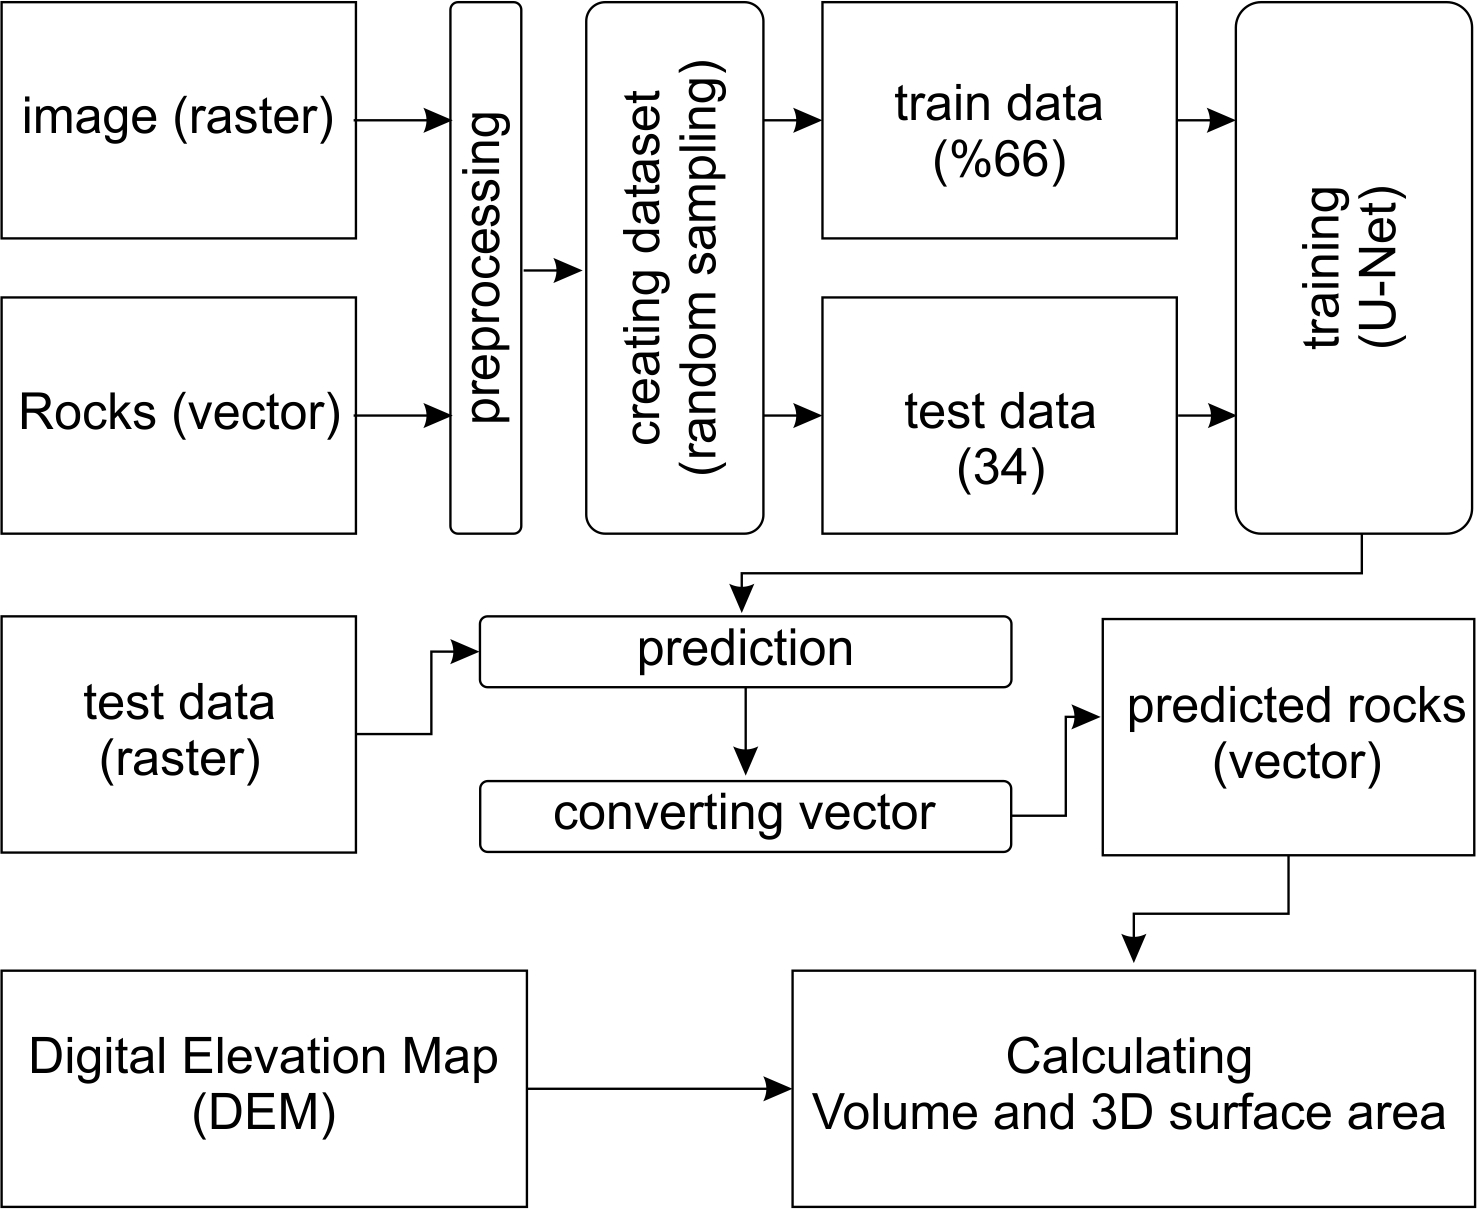
\includegraphics[width=0.75\textwidth]{figures/fig3.jpg}
	\caption{ Workflow diagram}
	\label{fig:Figure3}
\end{figure}
\subsection{Data preparation}
In this study required data was collected by UAV. DJI phantom 3-Pro was used for image acquisition. First, the area to be flown is determined, then the necessary parameters for image acquisition are entered by the Pix4d Capture software. These parameters were chosen as follows.\\
– Flight altitude (altitude): 100 m.\\
– Flight speed (speed): Fast\\
– Camera angle (Angle): 70$^o$\\
– Overlap: 80\%\\

The flight was carried out by the "Double Grid" method. The model of UAV used in this study does not have an obstacle detecting feature. Therefore, when determining the height, it is necessary to pay attention to the nearby power lines, tall buildings, trees, and peaks of hills.

The camera model (FC00X) of UAV has 4000$\times$3000 resolution, 3.61 mm focal length and 1.56$\times$1.56 µm pixel dimensions. After the flight, 284 images were obtained, and these images were processed with the Pix4Dmapper software. As a result, an orthophoto image with a resolution of 3.51 cm/pixel and a dimension of 2329$\times$1587 was created.

A region was selected from a large orthophoto image to create training and testing images. This area was chosen randomly. All visible rocks in the image were outlined using GIS software. The resulting file was saved as a vector file and used as mask data in the segmentation process. Following this, image and mask files were created separately.

A deep learning model requires the same-sized images. That's why a single image needs to be split into patches. The patch dimension was used as 256$\times$256. Train-test splitting rate was selected as 66\% for training data and 34\% for testing data. The large image was split into 9 parts to avoid sampling from the same regions. Areas 1,5, and 9 were selected for creating test images. Train images were selected from the other (2,3,4,6,7,8) areas (Fig. \ref{fig:Figure4}). A total of 560 images (256$\times$256) were selected, 369 images for training and 191 images for testing. The same processes were applied to extract the mask images.
\begin{figure}
	\centering
	\includegraphics[width=0.75\textwidth]{figures/fig4.jpg}
	\caption{ Train and test sampling areas. 1,5,9 test sampling area and 2,3,4,6,7,8 train sampling area}
	\label{fig:Figure4}
\end{figure}

The Albumentations \citep{buslaev2020albumentations} method was also used for data augmentation during the model-building stage. Albumentations includes many transform methods. The augmentation methods listed below were applied:\\
– horizontal flip\\
– affine transforms\\
– perspective transforms\\
– brightness/contrast/colours manipulations\\
– image blurring and sharpening\\
– gaussian noise\\

\subsection{Model building}
In this study, U-Net architecture \citep{ronneberger2015u} was used as segmentation model. This architecture is a type of fully convolutional network developed for biomedical image segmentation. It is named U-Net because the shape of the architecture is like the letter U. The network architecture of U-Net is shown in Fig. \ref{fig:Figure5}. It consists of two parts: contracting path (left side) and expanding path (right side). The first part captures context, and the second part enables precise localization. The left side consists of four blocks and each block contains two 3$\times$3 convolution layers + activation function (with batch normalization) and one 2$\times$2 max-pooling layer. Also, the right side consists of four blocks. These blocks include the steps of deconvolution layer, merging with feature map from subsampling path, 3$\times$3 convolution layer + activation function (with batch normalization). Finally, an additional 1$\times$1 convolution operation is applied to reduce the feature map to the required number of channels and generate the segmented image.
\begin{figure}
	\centering
	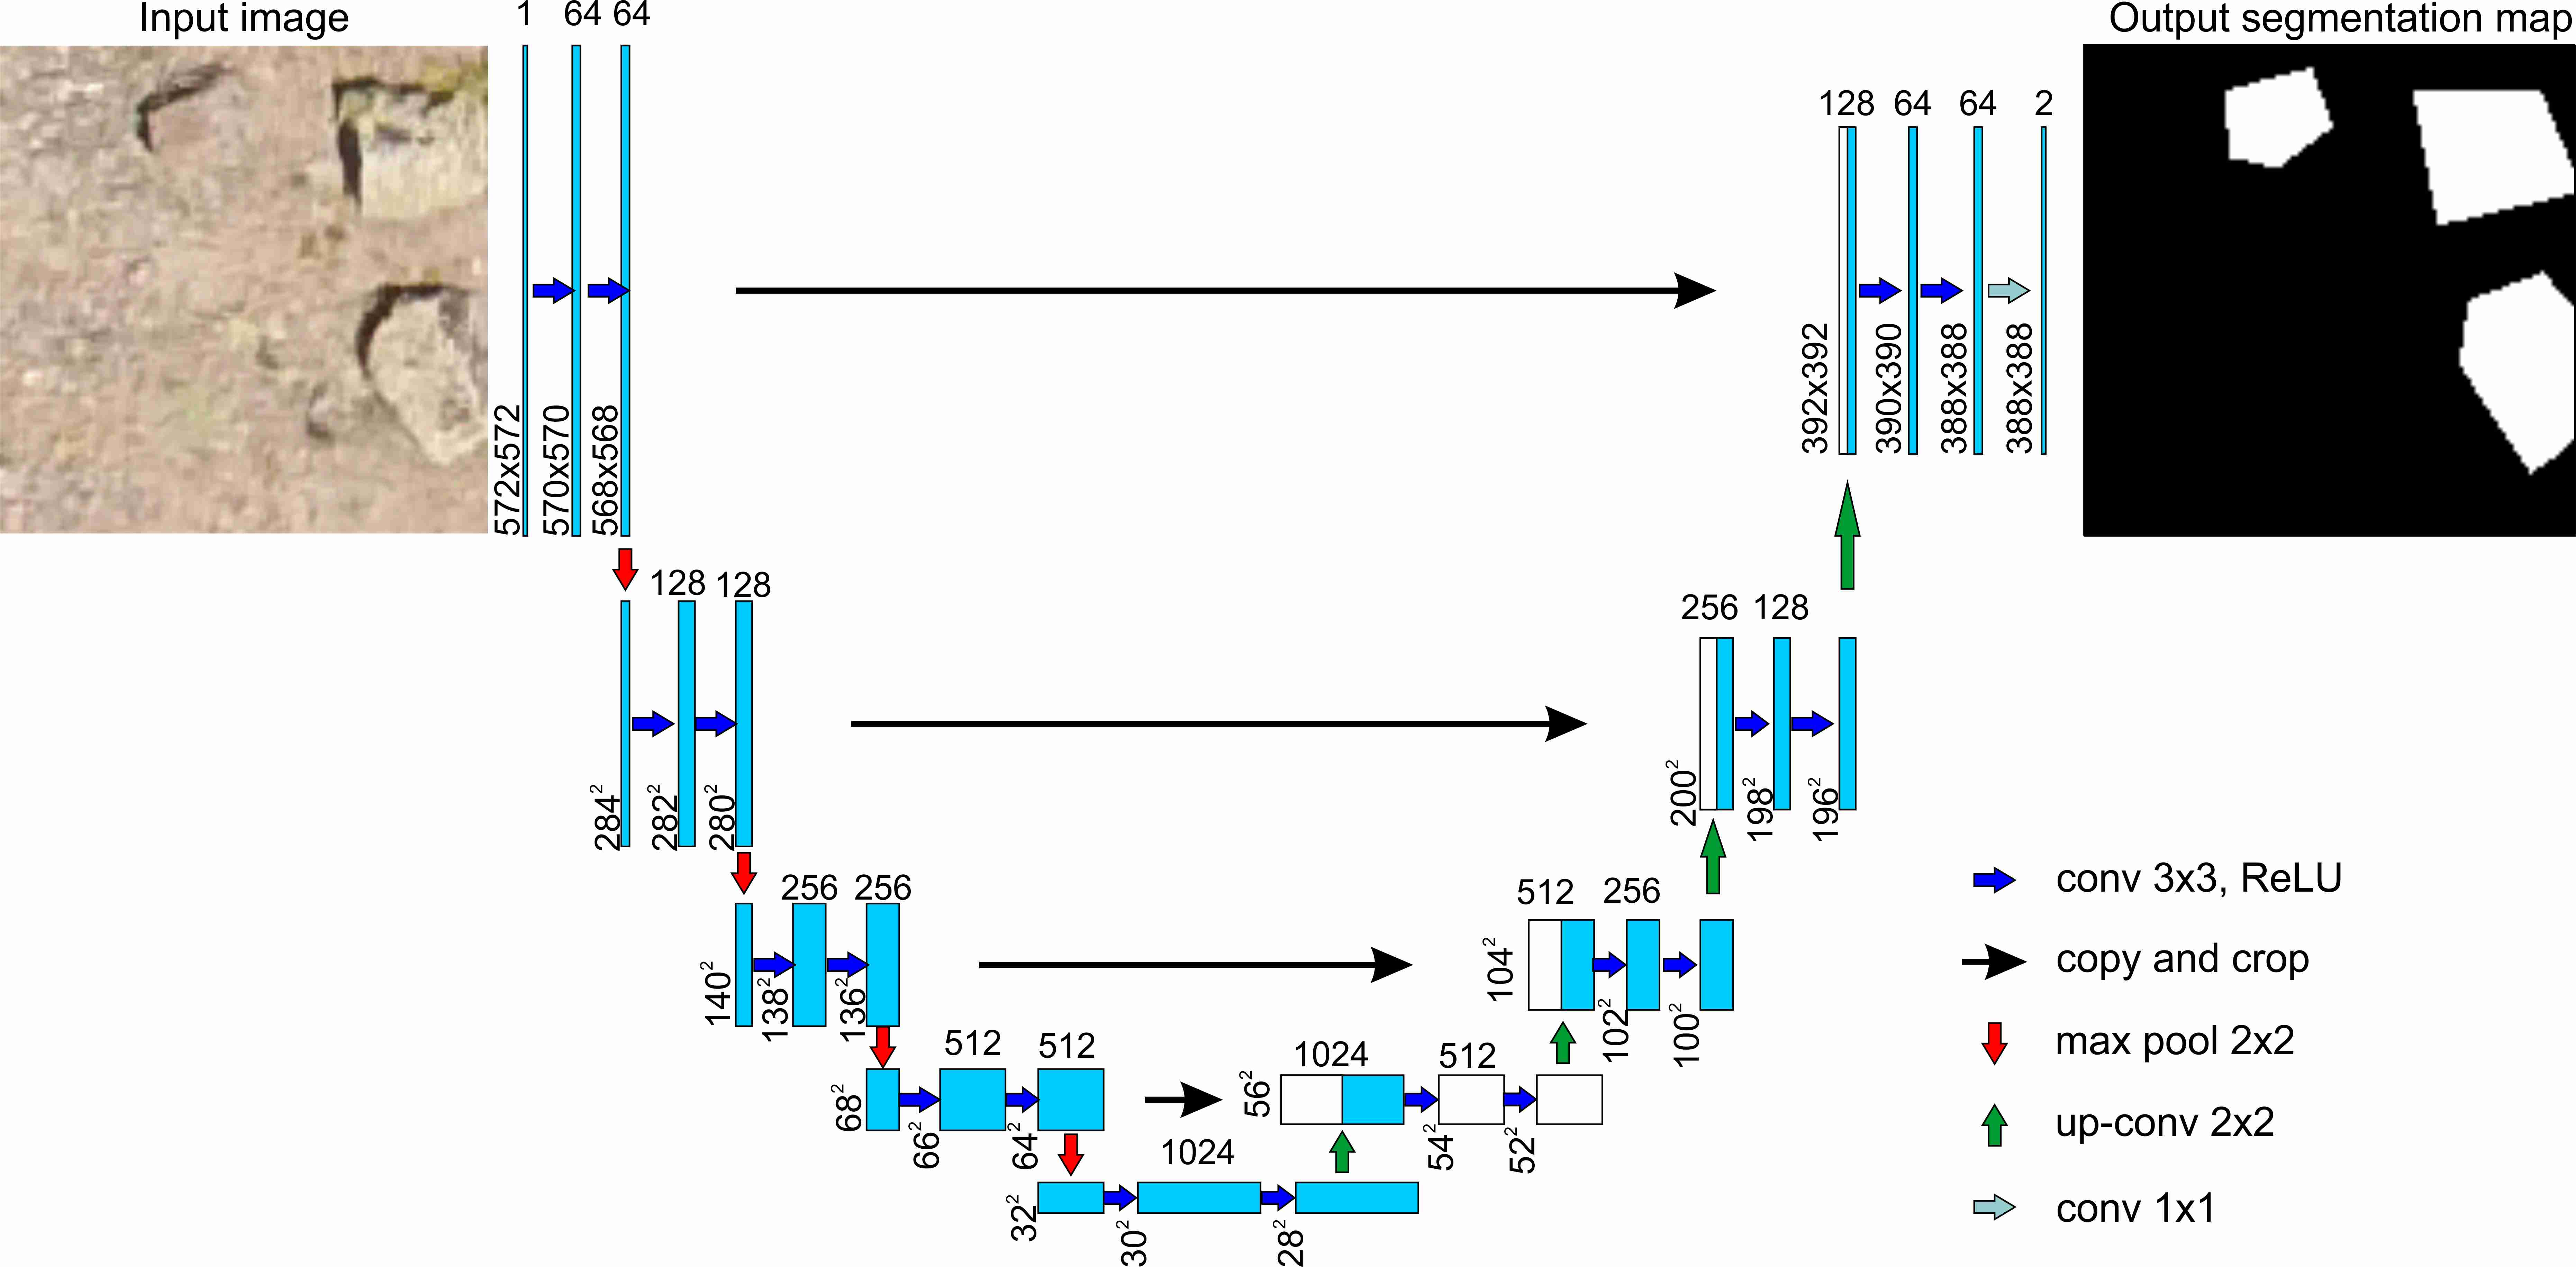
\includegraphics[width=0.75\textwidth]{figures/fig5.jpg}
	\caption{U-Net architecture}
	\label{fig:Figure5}
\end{figure}

DenseNet121 transfer learning model was used for feature extraction and rock segmentation was performed with U-Net. Segmentation model was evaluated in terms of IoU and F1-score metrics. IoU, which is frequently preferred in segmentation problems, is also known as the Jaccard similarity coefficient \citep{jaccard1912distribution}. It is the ratio of correctly classified pixels to the sum of the number of pixels in that class and the predicted number of pixels( Equation \ref{eqn:eq1}). 

\begin{equation}
\label{eqn:eq1}
    J(A,B) = \frac{|A \cap B|}{|A \cup B|}
\end{equation}
The F1-Score is important in that it is not False Negative or False Positive, but a measurement metric that includes all error costs. It is the harmonic mean of Precision and Recall values (Equation \ref{eqn:eq2}).

\begin{equation}
\label{eqn:eq2}
F1\text{-}Score = \frac{2 \times \text{Precision} \times \text{Recall}}{\text{Precision} + \text{Recall}}
\end{equation}

\begin{equation}
\label{eqn:eq3}
\text{Precision} = \frac{TP}{TP + FP}
\end{equation}

\begin{equation}
\label{eqn:eq4}
\text{Recall} = \frac{TP}{TP + FN}
\end{equation}
Where TP is True Positive, FP is False Positive and FN is False Negative.


\section{Results}
In this study, we created our own dataset. A large orthophoto image with a dimension of 2329$\times$1587 was created from UAV images. This image needs to be patched for use in the segmentation model. A python script has been written for this purpose. It is possible to create the desired number and size of images with the written script. Random corner coordinates with the size of 256$\times$256 patches were created. Obtaining images with the exact corner coordinates was prevented. Because of this condition, the program gives an error when too many images are wanted to be created. Also, the probability of creating very similar images increases. Using the grid method, 56 images can be obtained from the large orthophoto image. Using the random sampling method 560 images were obtained from the same image.

U-Net segmentation model was used with DenseNet121. IOU and F1-score were used as performance metrics. The model was trained and tested with different parameters. The parameters providing the best results are given in Table\ref{tab:Table1} below.


\begin{table}
	\centering
	\caption{Model parameters}
	\label{tab:Table1}
	\begin{tabular}{ |c|c|} 
		\hline
		Optimizer&Adam\\ 
		\hline 
		Learning rate&0.0001\\
		\hline
		Batch size&8\\
		\hline
		Image size&256$\times$256\\
		\hline
		Epoch&100\\
		\hline
	\end{tabular} 
\end{table}


IoU scores and losses graph of model are shown in Figure \ref{fig:Figure6}. The results of the model are satisfactory for the segmentation task. Train IoU, test IoU, train F1-score and test F1-score were calculated as 0.85\%, 0.85\%, 0.92\%, and 0.92\%, respectively.

\begin{figure}
	\centering
	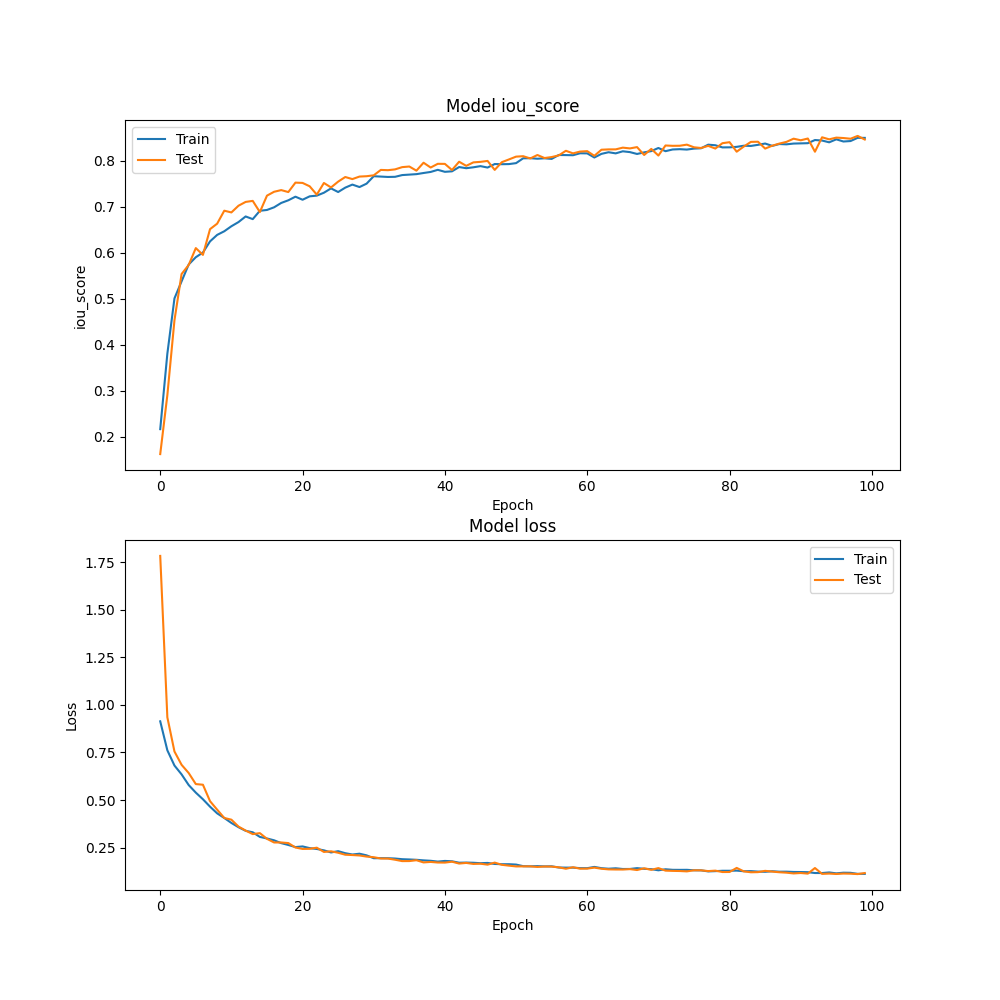
\includegraphics[width=0.75\textwidth]{figures/fig6.png}
	\caption{DenseNet121 IoU and Loss values}
	\label{fig:Figure6}
\end{figure}

The trained model successfully detected rock blocks within the study area (Fig. \ref{fig:Figure7}). The boundaries of 3111 rocks of various sizes were determined and created as a vector file (.shp). This detection method is not recommended for smaller areas. Because sufficient training data cannot be created. In areas where there are several rock blocks, detection can also be done manually. 
Sometimes there may be distortions at the edges and corners of the image. This causes errors in rock block detection. Therefore, a larger area than the area where the rocks are located should be selected as the study area.

\begin{figure}
	\centering
	\includegraphics[width=0.75\textwidth]{figures/fig7.jpg}
	\caption{Result map of the model (a) original view, (b,c,d )zoomed views.}
	\label{fig:Figure7}
\end{figure}

After the rocks were detected, each rock's volume and 3D surface area were calculated. These calculations were performed using Python. Calculated values were saved in the shape file as fill volume, cut volume and 3D area.

In volume calculations, there must be a reference height or surface. In this study, the heights at the boundaries of the rocks were selected as the reference height. The calculations were made using an image containing elevation data. This image consists of pixels containing elevation values, which are organized into rows and columns. The elevation values in each row were used to calculate the total volume. The polygons showing the boundaries of the rocks were masked with elevation data. Thus, data with elevation values for each rock were obtained. Volumes were calculated by proceeding along the rows. The slope was calculated by comparing the elevation values at the beginning and end of the row. A new base elevation was determined for each pixel and the volumes were calculated from this elevation.

In this method, it is necessary to evaluate three different scenarios. In the first case, the first and last elevations of the rows are equal. Here, the starting elevation value is used as the reference height. Volumes above this elevation are calculated as fill volumes, while volumes below are calculated as cut volumes. In the second case, the first elevation is greater than the last elevation of the rows. In the third case, the first elevation is less than the last elevation of the rows. Different calculations are required for each scenario. These situations are illustrated in Figure \ref{fig:Figure8}.
\begin{figure}
	\centering
	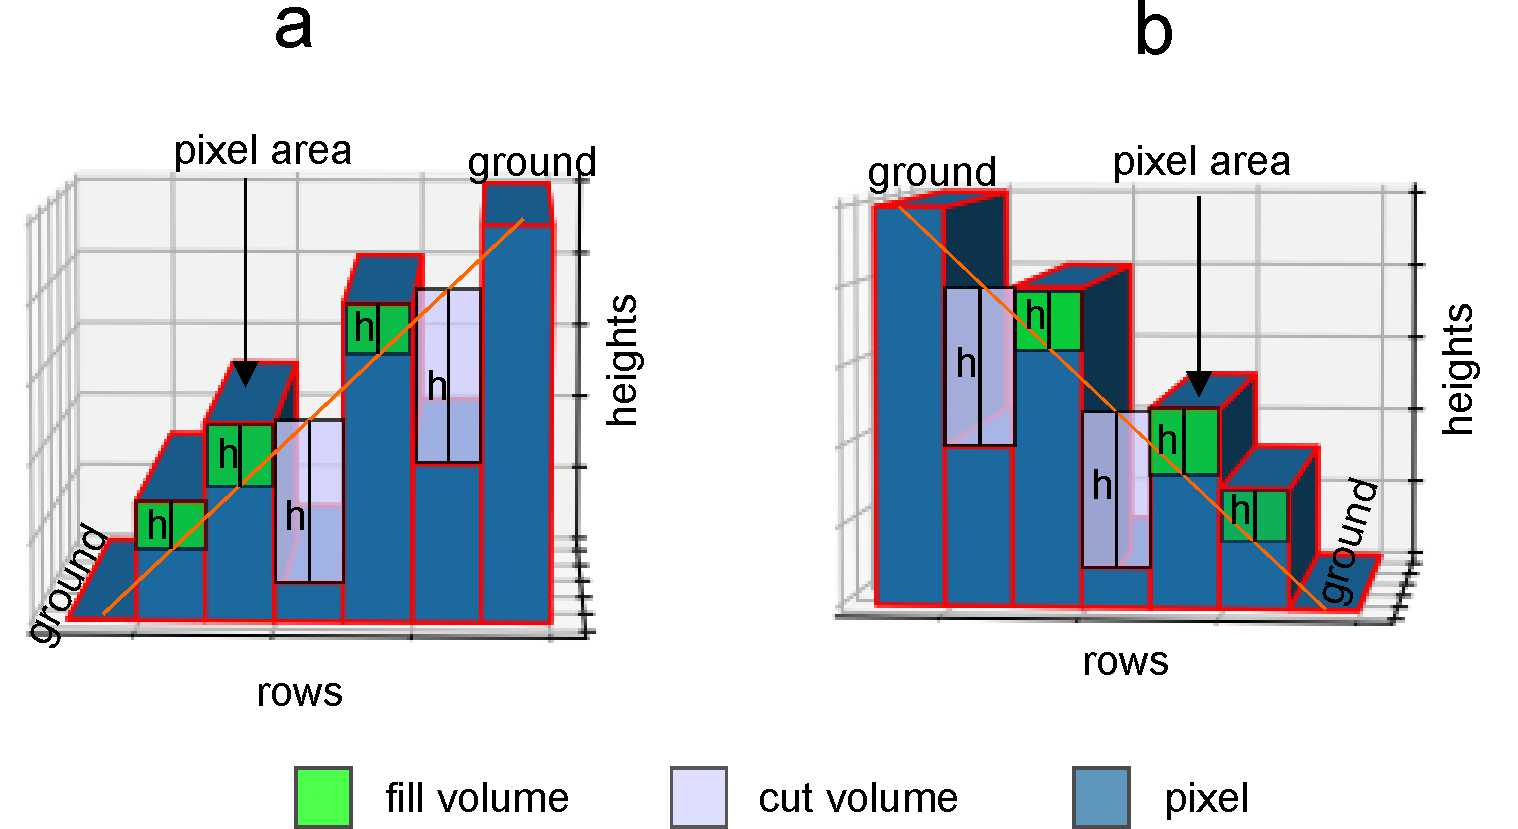
\includegraphics[width=0.75\textwidth]{figures/fig8.jpg}
	\caption{Volume calculation methods. (a) first height is greater than the last height of the rows,(b) b) first height is less than the last height of the rows}
	\label{fig:Figure8}
\end{figure}

Volume calculation can be easily done by multiplying the pixel area by the height. Heights need to be calculated for each pixel. The starting and ending pixels along a row are assumed to be ground. These ground elevations are used to find the slope, and each pixel's height is recalculated using this slope. Fill volume and cut volume were calculated using new heights and pixel areas. Slopes, fill volumes and cut volumes were determined using the method in Figure \ref{fig:Figure8}. The total volumes (fill and cut) are found by summing the calculations made for each row.

The 3D surface area was calculated by Python script. Calculations of flat surfaces can be found by multiplying pixel lengths. However, different methods must be used for irregular surfaces. The gradient method was used in 3D surface calculation. Height changes were calculated in X and Y directions, gradient vectors were obtained in each direction. Surface areas were calculated by using these vectors. The slope correction equation is used to determine the sloped surfaces (Equation \ref{eqn:eq5}).

\begin{equation}
\label{eqn:eq5}
\text{slope correction} = \sqrt{1 + \left(\frac{\partial z}{\partial x}\right)^2 + \left(\frac{\partial z}{\partial y}\right)^2}
\end{equation}

\begin{equation}
\label{eqn:eq6}
\frac{\partial z}{\partial x} = \text{gradient in X direction}, \quad \frac{\partial z}{\partial y} = \text{gradient in Y direction}
\end{equation}

The 3D surface area is calculated as following:
\begin{equation}
\label{eqn:eq7}
\text{3D surface area} = \sum \text{pixel area} \times \text{slope correction}
\end{equation}


\section{Conclusions}

This study aims to segment rock blocks and calculate the volume and 3D surface areas of the blocks obtained as a result of segmentation. The methods used in the segmentation process provided the determination of the boundaries of rock blocks with high accuracy rates. In this way, the geometric properties of the blocks were analysed in detail.

U-Net deep learning network and DenseNet121 model were used as segmentation methods. The boundaries of rock blocks were determined accurately with the trained model.

The volume of each rock block was successfully calculated from the data obtained after segmentation. Similarly, the 3D surface areas of the blocks were calculated. High-resolution Digital Elevation Map (DEM) data were used in volume and surface area calculations. Determination of block volumes and 3D surface areas is of critical importance, especially for rockfall simulations and engineering analyses. In addition, since the outputs of the study are coordinated vector data, they can be easily used in any GIS software. It can be a basis for different studies and analyses.

This study has presented a reliable method for segmentation and volume/surface area calculations and has also directly contributed to engineering applications in terms of determining the physical properties of rock masses. The segmentation section of the study is recommended for terrains containing a lot of rock blocks. It is possible to detect rock blocks in a short time. In addition, this method can be used to automatically detect different types of terrain. This study requires DEM and orthophoto images obtained from the field. A region is selected and labelled objects in any GIS software for training the model. The following processes are carried out entirely with Python scripts.

Deep learning models usually require a large amount of data for training. A large amount of data can be generated with the Random Sampling method proposed in this study. Volume and 3D surface area algorithms can be used not only for rock blocks but also for any object on the field. These algorithms only require precise DEM data and object boundaries. For example, these calculations can be made for a single rock block. In these calculations, ground heights and object heights must be determined clearly. When determining the object boundaries, they should be extended towards the ground. If the boundaries only represent the object, the ground heights will not be considered, and the results will not be correct. In some cases, the model can draw the boundaries of the rock blocks narrower. In this case, this problem can be solved by adding buffers to the rock blocks.

As a result, this study provides a basis for volumetric and geometric analyses for rock mechanics, geology and engineering applications, and can be expanded by testing on different rock types and fields in future studies.


\section{Acknowledgments}

The author wants to thank the Prime Ministry Disaster and Emergency Management Authority for supplying orthophoto images and geological map.

\newpage

\textbf{Code availability section}

Name of the code: rock\_segmentation

Contact: ali.polat@afad.gov.tr

Program language: Python
 
Software required: Python v3.9

Program size: 35.7 KB

The source codes are available for downloading at the link:
https://github.com/apolat2018/rock\_segmentation


\bibliographystyle{cas-model2-names}
\bibliography{bibliography} 

\end{document}

